\chapter{Machine Learning}
\label{sec:ml}
The scientific field of \acrfull{ml} if often seen as a part of the greater field of \acrfull{ai}\cite[3]{Alpaydin10}, and the term was coined by Arthur Samuel in \citeyear{samuelmachinelearning} \cite{samuelmachinelearning}. An \acrshort{ml} algorithm builds a model based on a dataset, with the goal of making predictions or classifications without being explicitly programmed how to do so. 

Some problems can easily be solved by programming an explicit algorithm (e.g. sorting a list, or \acrshort{fbp} reconstruction), however there are many cases where an exact algorithm simply does not exist (e.g. telling spam emails from legitimate emails) \cite[1]{Alpaydin10}. Often we have access to a large amount of sample data (e.g. emails where some have been manually flagged as spam) pertaining to the issue, however what is lacking is a suitable algorithm to parse and classify all the data. This is where \acrshort{ml} comes in: an \acrshort{ml} model can be trained to discern differences in a dataset without being explicitly told what to look for. So long as there is a sufficient amount of data to train the model with, it may be able to find a pattern in the data and thereby augment or enhance the data, or predict or classify new data \cite[2-4]{Alpaydin10}. 

There are many different \acrshort{ml} algorithms, however in this thesis only the class of neural networks will be discussed and the focus will be on supervised learning. 

\section{Components of a Neural Network}
Neural networks were initially designed to simulate the human brain and how it learns and adapts to new information \cite{McCulloch1943}. Because of this, the basic building block of a neural network is called a neuron. Several neurons builds up a layer, and several layers build up a neural network. Neurons in different layers have connections to each other (i.e. neurons in layer 1 are connected to neurons in layer 2), and these connections have weights and biases. A simple schematic of this can be seen in \cref{fig:neuralnetwork}. The value of a neuron is a real number, and can be given as \cite[81]{Wang2003}
\begin{equation}
    \label{eq:neuron}
    Y_{k} = \sigma\left(\sum_{j=0}^{m}w_{kj}x_j + \lambda \right),
\end{equation}
where $k$ refers to which neuron it is, $m$ is the number of inputs to the neuron, $w_{kj}$ is the weight of connection $j$, $x_j$ is the output value of neuron $j$ into neuron $k$, $\lambda$ is a bias term, and $\sigma$ is the activation (or transfer) function, which will be introduced later. It is thus a weighted sum of the values of the neurons in the previous layer (or more precisely, of all the input neurons to a given neuron, which often is the previous layer). Note that this describes a simple \acrfull{ann}, and other types of neural networks may contain other types of layers. \todo[]{Cite sources for this paragraph}

\begin{figure}[htbp]  
    \centering
    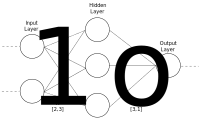
\includegraphics[width=.8\textwidth]{figures/neuralnetwork.pdf}
    \caption[Neural network example]{A simple schematic of a neural network. Each circle represents a neuron, the solid arrows represent connections between neurons, and the dotted arrows represent input and output channels. The dimensions of the network parameters are denoted as $W_n$, where $n$ refers to the output layer of the parameters. This network speifically is a fully connected feedforward \acrlong{ann} with one hidden layer. }
    \label{fig:neuralnetwork}
\end{figure}

The activation function, also known as the transfer function, is denoted as $\sigma$. Its purpose is to bound the value of a neuron so that the network is not crippled by divergent neurons \cite[81]{Wang2003}. There are many different activation functions, and some examples are presented in \cref{tab:activationfunctions} and plotted in \cref{fig:activationfunctions}. Furthermore, the activation function is used to introduce nonlinearity to the network\footnote{For this reason, the identity activation function $f(x)=x$ generally performs poorly.}, and it can be shown that a two-layer deep neural network with a nonlinear activation function is a universal function approximator \cite{Cybenko1989}. 

\begin{table}[htbp]
    \centering
    \caption[Activation functions]{Overview of some of the commonly used activation functions in neural networks. }
    \label{tab:activationfunctions}
    \begin{tabular}{ll}
    \hline
    Name & Function, $f(x)$ \\
    \hhline{==}
    Identity & $x$ \\
    Logistic/soft step & $\frac{1}{1+e^{-x}}$  \\
    Rectified Linear Unit (ReLU) & $\max\left(0, x\right)$ \\
    Leaky Rectified Linear Unit (LReLU) & $\max\left(\alpha x, x\right), \alpha\in[0,1]$ \\
    tanh & $\frac{e^x - e^{-x}}{e^x + e^{-x}}$ \\
    Softplus & $\ln\left(1+e^x\right)$ \\
    \hline
    \end{tabular}
\end{table}

\begin{figure}[htbp]  
    \centering
    \includegraphics[width=.8\textwidth]{figures/activationfunctions.pdf}
    \caption[Activation functions]{Plot showing a selection of activation functions for $x\in[-2,2]$. Note that identity, ReLU, and LReLU are overlapping for $x\in[0,-2]$. }
    \label{fig:activationfunctions}
\end{figure}

The output of a neural network can be defined to be any shape. Depicted in \cref{fig:neuralnetwork} the output is a singular value, however it could just as well have been defined as a vector of two values. If the output is a singular value it can for instance be interpreted as a probability, however if it is a vector of length $n$ it can be seen as $n$ probabilites of different events. The output of a neural network is often called a feature map, because it can be seen as a mapping of the features of the input data. 

As an example, if a neural network is trained with a dataset containing images of handwritten digits $0-9$, an output with a size of $10$ could contain probabilities of a given image containing a specific digit where each output value is the probability of one digit. One well-known dataset that is often used for this exact problem is the MNIST dataset \cite{mnist}.

\todo[inline]{Maybe own section on hyperparameters? If not, make subsection}


\section{Neural Network Types}


\subsection{Artificial Neural Network}
Linear function $ax+b$, and a non-linear activation function $\sigma$. 

Affine transformations and pointwise nonlinearities which are smooth Lipschitz functions (such as sigmoid, tanh, elu, softplus, etc.). 

\subsection{Convolutional Neural Network}
Convolutional kernels. Useful for image processing. Extract spatial information, context. Fewer parameters to train

\subsection{Encoder-Decoder Network}
Downscaling and upscaling between layers, and skip connections (for U-net, but not actually in encoder-decoder networks). % https://www.researchgate.net/post/Are_U-net_and_encoder-decoder_network_the_same 

\subsection{Generative Adversarial Network}
Learn probability distribution and generate random sample from learned distributiom. 
GAN based on game theory instead of optimization. 

\section{Training a Neural Network}
The process of tuning all the parameters (i.e. weights and biases) of a neural network is called training. During training, input data from a training dataset is forwards propagated through the network, and the resulting feature map is compared to an expected feature map (e.g. manually labeled data)\footnote{This is what is called supervised learning, as opposed to unsupervised learning where there is no ground truth answer to compare to. }. The difference in these feature maps is calcuated using some loss function, and the loss is then backwards propagated through the network to update each and every parameter to reduce the loss. 

Generally, the entire training dataset is repeatedly passed through the network multiple times. Each full runthrough of the training dataset is called an epoch of training. This however can often introduce a problem: the training dataset can typically not fully fit in the computer memory at once. Therefore it is divided into mini batches, and after each mini batch the weights are adjusted. The propagation of one mini batch is often called one iteration, and thus one epoch consists of several iterations. The size of a mini batch is a tunable parameter, however typically it is in the range of $32-512$ (e.g. 128 in the well-known article by A. Krizhevsky et al. \cite{alexnet})\footnote{There is ongoing research into techniques to increase the batch size by several orders of magnitude as larger batches allow for easier parallelization, however large batch sizes have been shown to cause instability during training \cite{you2017large}. }. The size of a mini batch can sometimes also be refered to as the batch size. 

\subsection{Hyperparameters}
During training, the parameters of the neural network are automatically changed, however there are some parameters that are set manually beforehand. These are called hyperparameters. Some typical hyperparameters are:
\begin{itemize}
    \item Number of layers (i.e. depth of network).
    \item Size of layers.
    \item Learning rate.
    \item Number of iterations to train the network (i.e. number of epochs).
    \item Mini batch size.
\end{itemize}

The process of choosing these hyperparameters is not an exact science, and there is much research being done into finding ways of automatically tuning hyperparameters to their ideal configurations, called auto-tuning \cite{autotuning}.

\subsection{Loss Functions}
MSE, MAE, LogCosh, VGG, Adversarial, 


\subsection{Backpropagation}


\subsection{Optimizers}

\subsubsection{Stochastic Gradient Descent}
Article: \cite{stochasticgradientdescent}

\subsubsection{ADAM}
Article: \cite{kingma2015adam}
